\documentclass{beamer}
\usetheme{metropolis}           % Use metropolis theme

\metroset{numbering=none}
\setmonofont{Fira Code}

\usepackage{minted}
\usemintedstyle{friendly}
\setminted{
    frame=none, %lines,
    framesep=2mm,
    baselinestretch=1.2,
    %bgcolor=lightgray,
    fontsize=\footnotesize,
    escapeinside=\#\#
    }
\usepackage{filecontents}

\usepackage{tikz}

\definecolor{bg}{rgb}{0.85,0.85,0.85}

\metroset{background=dark}

\usebackgroundtemplate{%
\tikz[overlay,remember picture] \node[at=(current page.center), opacity=0.5] {
   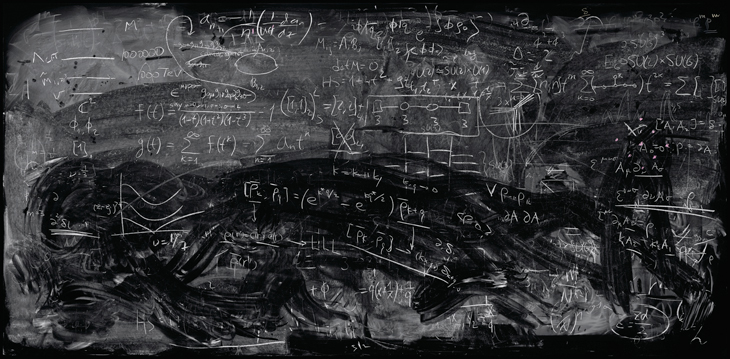
\includegraphics[height=\paperheight]{alejandro_guijarro_StanfordI}};
}

\title{Safe APIs from Ghosts of Departed Proofs}
\date{\today}
\author{Matt Noonan}
\institute{Kataskeue LLC \& Input Output HK}
\begin{document}
\maketitle

\usebackgroundtemplate{}

\begin{frame}{Micro-intro}
  one slide
\end{frame}

%%%%%%%%%%%%%%%%%%%%%%%%%%%%%%%%%%%%%%%%%%%%%%%%%%%%%%%%%%%%%%%%%%%%%%%%
  \section{How do we make good APIs?}   %%%%%%%%%%%%%%%%%%%%%%%%%%%%%%%%
%%%%%%%%%%%%%%%%%%%%%%%%%%%%%%%%%%%%%%%%%%%%%%%%%%%%%%%%%%%%%%%%%%%%%%%%

  \begin{frame}f
    In par
\end{frame}
  
\begin{frame}{Unsafe strategy: explode}
  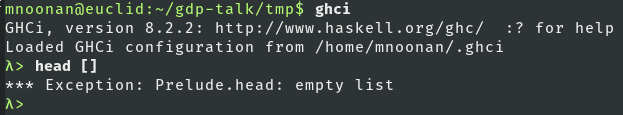
\includegraphics[width=0.8\paperwidth]{hsout}
\end{frame}

\begin{frame}{Unsafe strategy: explode?}
  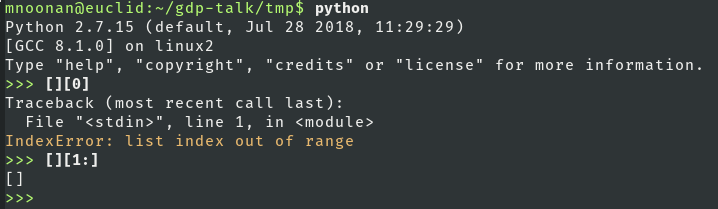
\includegraphics[width=0.8\paperwidth]{pyout}
\end{frame}

%%%%%%%%%%%%%%%%%%%%%%%%%%%%%%%%%%%%%%%%%%%%%%%%%%%%%%%%%%%%%%%%%%%%%%%%
\begin{frame}{Unergonomic strategy: special value}
  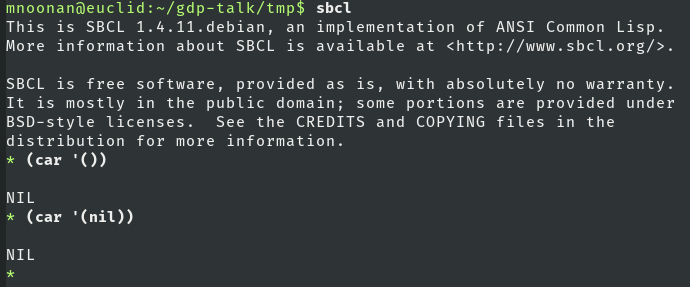
\includegraphics[width=0.8\paperwidth]{lispout}
\end{frame}


%%%%%%%%%%%%%%%%%%%%%%%%%%%%%%%%%%%%%%%%%%%%%%%%%%%%%%%%%%%%%%%%%%%%%%%%

\begin{frame}{Unpalatable strategy: anything goes}
  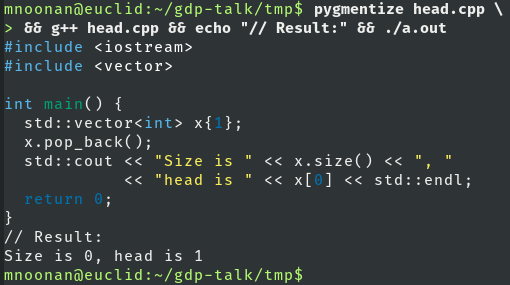
\includegraphics[width=0.8\paperwidth]{cppout}
\end{frame}

%%%%%%%%%%%%%%%%%%%%%%%%%%%%%%%%%%%%%%%%%%%%%%%%%%%%%%%%%%%%%%%%%%%%%%%%
\begin{filecontents*}{safehead.hs}
data NonEmptyList a = NonEmptyList a [a]
  
headNE :: NonEmptyList a -> a
headNE (NonEmptyList x xs) = x  
\end{filecontents*}
\begin{frame}{Safe idiom: refinement types to restrict domain}
  \inputminted{haskell}{safehead.hs}
\end{frame}

%%%%%%%%%%%%%%%%%%%%%%%%%%%%%%%%%%%%%%%%%%%%%%%%%%%%%%%%%%%%%%%%%%%%%%%%

\begin{filecontents*}{headmay.hs}
headMay :: [a] -> Maybe a
headMay = \case
    []     -> Nothing
    (x:xs) -> Just x
\end{filecontents*}
\begin{frame}{Safe idiom: option types to expand range}
  \inputminted{haskell}{headmay.hs}
\end{frame}

\begin{filecontents*}{headdt.agda}
head : #$\forall$# {A n} → Vec A (1 + n) → A
head (x :: xs) = x

zip : #$\forall$# {A B n} → Vec A n → Vec B n → Vec (A × B) n

take : #$\forall$# {A} m {n} → Vec A (m + n) → Vec A m
\end{filecontents*}
\begin{frame}{Safe idiom: say what you mean with dependent types}
  \inputminted{agda}{headdt.agda}
\end{frame}

%%%%%%%%%%%%%%%%%%%%%%%%%%%%%%%%%%%%%%%%%%%%%%%%%%%%%%%%%%%%%%%%%%%%%%%%
  \section{Idea}   %%%%%%%%%%%%%%%%%%%%%%%%%%%%%%%%%%%%%%%%%%%%%%%%%%%%%
%%%%%%%%%%%%%%%%%%%%%%%%%%%%%%%%%%%%%%%%%%%%%%%%%%%%%%%%%%%%%%%%%%%%%%%%

\begin{filecontents*}{sortby.hs}
sortBy  :: (a -> a -> Ordering) -> [a]        -> [a]
mergeBy :: (a -> a -> Ordering) -> [a] -> [a] -> [a]

-- BE CAREFUL! xs and ys must already be sorted by comp!
mergeBy comp xs ys = case (xs, ys) of
    (_, []) -> xs
    ([], _) -> ys
    ((x:xs'), (y:ys')) -> case comp x y of
        LT -> x     : mergeBy comp xs' ys
        GT ->     y : mergeBy comp xs  ys'
        EQ -> x : y : mergeBy comp xs' ys'
\end{filecontents*}
\begin{frame}{A finicky API}
\inputminted{haskell}{sortby.hs}    
\end{frame}

%%%%%%%%%%%%%%%%%%%%%%%%%%%%%%%%%%%%%%%%%%%%%%%%%%%%%%%%%%%%%%%%%%%%%%%%

\begin{filecontents*}{mergemay.hs}
module FancySafeMerge where
  
mergeMay :: (a -> a -> Ordering) -> [a] -> [a] -> Maybe [a]
mergeMay comp xs ys =
    if isSorted xs && isSorted ys
      then Just (mergeBy comp xs ys)
      else Nothing
  where
    isSorted (z : zs@(z' : _)) =  comp z z' /= GT
                               && isSorted zs
    isSorted _ = True
\end{filecontents*}
\begin{frame}{Can we make it safe with optional types?}
\inputminted{haskell}{mergemay.hs}
\end{frame}

%%%%%%%%%%%%%%%%%%%%%%%%%%%%%%%%%%%%%%%%%%%%%%%%%%%%%%%%%%%%%%%%%%%%%%%%
\usebackgroundtemplate{%
\tikz[overlay,remember picture] \node[at=(current page.center)] {
   
\includegraphics[height=\paperheight]{angel}};
}
\begin{frame}{}\end{frame}
\usebackgroundtemplate{}

\begin{frame}{}
  \center{\Large{\textbf{No.}}}
\end{frame}

\usebackgroundtemplate{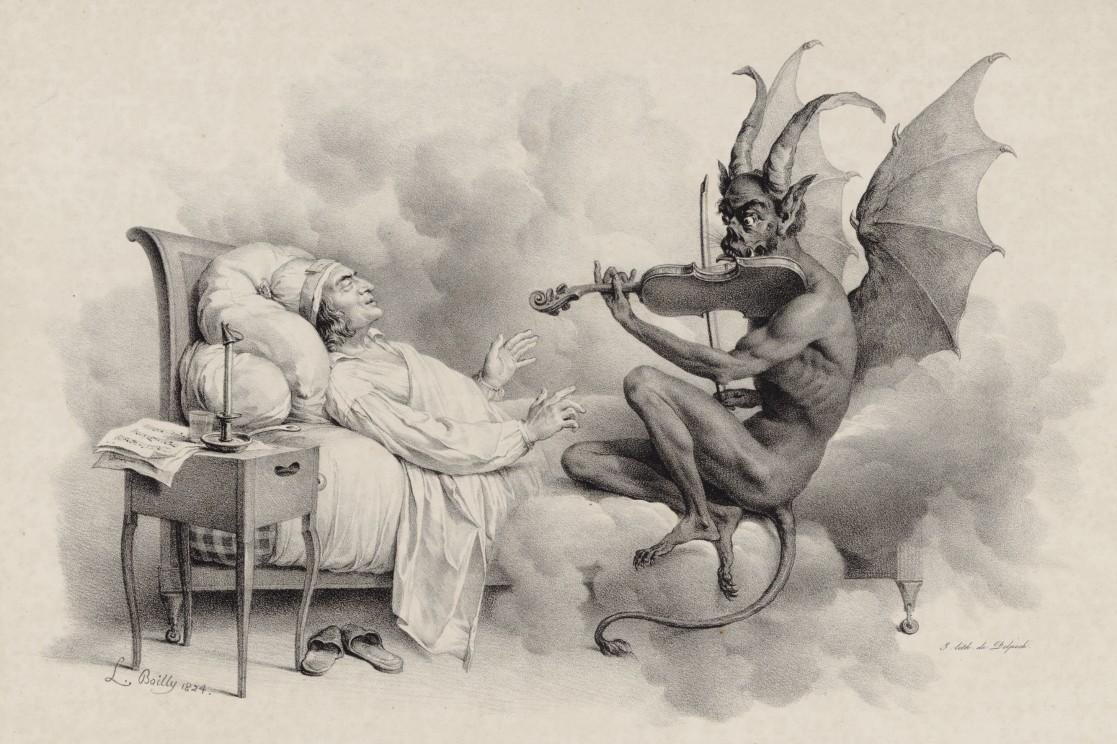
\includegraphics[width=\paperwidth,height=\paperheight]{tartinis-dream}}
\begin{frame}{}\end{frame}
\usebackgroundtemplate{}

\begin{filecontents*}{median.hs}
import FancySafeMerge

median :: [Int] -> [Int] -> Int
median xs ys = merged !! midpt
  where
    xs'    = sortBy compare xs
    ys'    = sortBy compare ys
    merged = fromJust (mergeMay compare xs' ys')
    midpt  = length merged `div` 2
\end{filecontents*}
\begin{frame}{Leading the user into sin and vice}
\inputminted{haskell}{median.hs}
\end{frame}

%%%%%%%%%%%%%%%%%%%%%%%%%%%%%%%%%%%%%%%%%%%%%%%%%%%%%%%%%%%%%%%%%%%%%%%%

%%%%%%%%%%%%%%%%%%%%%%%%%%%%%%%%%%%%%%%%%%%%%%%%%%%%%%%%%%%%%%%%%%%%%%%%
  \section{Overview}   %%%%%%%%%%%%%%%%%%%%%%%%%%%%%%%%%%%%%%%%%%%%%%%%%
%%%%%%%%%%%%%%%%%%%%%%%%%%%%%%%%%%%%%%%%%%%%%%%%%%%%%%%%%%%%%%%%%%%%%%%%

\begin{frame}{One}
\end{frame}

%%%%%%%%%%%%%%%%%%%%%%%%%%%%%%%%%%%%%%%%%%%%%%%%%%%%%%%%%%%%%%%%%%%%%%%%

\begin{frame}{Two}
\end{frame}

%%%%%%%%%%%%%%%%%%%%%%%%%%%%%%%%%%%%%%%%%%%%%%%%%%%%%%%%%%%%%%%%%%%%%%%%

\begin{frame}{Three}
\end{frame}

%%%%%%%%%%%%%%%%%%%%%%%%%%%%%%%%%%%%%%%%%%%%%%%%%%%%%%%%%%%%%%%%%%%%%%%%
  \section{Implementation}   %%%%%%%%%%%%%%%%%%%%%%%%%%%%%%%%%%%%%%%%%%%
%%%%%%%%%%%%%%%%%%%%%%%%%%%%%%%%%%%%%%%%%%%%%%%%%%%%%%%%%%%%%%%%%%%%%%%%

\begin{frame}{One}

\end{frame}

%%%%%%%%%%%%%%%%%%%%%%%%%%%%%%%%%%%%%%%%%%%%%%%%%%%%%%%%%%%%%%%%%%%%%%%%
\begin{frame}{Two}

\end{frame}

%%%%%%%%%%%%%%%%%%%%%%%%%%%%%%%%%%%%%%%%%%%%%%%%%%%%%%%%%%%%%%%%%%%%%%%%
\begin{frame}{Three}

\end{frame}

%%%%%%%%%%%%%%%%%%%%%%%%%%%%%%%%%%%%%%%%%%%%%%%%%%%%%%%%%%%%%%%%%%%%%%%%

\begin{frame}{Four}

\end{frame}

%%%%%%%%%%%%%%%%%%%%%%%%%%%%%%%%%%%%%%%%%%%%%%%%%%%%%%%%%%%%%%%%%%%%%%%%
\begin{frame}{Five}

\end{frame}

%%%%%%%%%%%%%%%%%%%%%%%%%%%%%%%%%%%%%%%%%%%%%%%%%%%%%%%%%%%%%%%%%%%%%%%%
\begin{frame}{Six}

\end{frame}

%%%%%%%%%%%%%%%%%%%%%%%%%%%%%%%%%%%%%%%%%%%%%%%%%%%%%%%%%%%%%%%%%%%%%%%%

\begin{frame}{Seven}

\end{frame}

%%%%%%%%%%%%%%%%%%%%%%%%%%%%%%%%%%%%%%%%%%%%%%%%%%%%%%%%%%%%%%%%%%%%%%%%
  \section{Examples}   %%%%%%%%%%%%%%%%%%%%%%%%%%%%%%%%%%%%%%%%%%%%%%%%%
%%%%%%%%%%%%%%%%%%%%%%%%%%%%%%%%%%%%%%%%%%%%%%%%%%%%%%%%%%%%%%%%%%%%%%%%

\begin{filecontents*}{hashes.hs}
newtype HashOf x = HashOf Defn

realHash :: Serializable a =>  a       ->  Hash
hash     :: Serializable a => (a ~~ x) -> (Hash ~~ HashOf x)

hash x = defn (realHash (serialize $ the x))

-- A type for objects along with their hash.
data ThingWithHash a = forall x. ThingWithHash
  { _thing :: a    ~~ x
  , _hash  :: Hash ~~ HashOf x }

-- Use it like this:
hashIt :: Serializable a => a -> ThingWithHash a
hashIt x = name x $ \x' ->
  ThingWithHash { _thing = x', _hash = hash x' }
                          
    
\end{filecontents*}

\begin{frame}{Hashed data structures}
\inputminted{haskell}{hashes.hs}
\end{frame}

\begin{filecontents*}{st2.hs}
-- Running an ST computation with shared regions
runSt2  ::
  STRef (forall mine yours. ST (mine #$\cap$# yours) a) -> a

inMine  :: ST mine  a -> ST (mine #$\cap$# yours) a
inYours :: ST yours a -> ST (mine #$\cap$# yours) a

-- Sharing an STRef we own
share  :: STRef mine a -> ST mine (STRef (mine #$\cap$# yours) a)

-- Using an STRef that was shared with us
use    :: STRef (mine #$\cap$# yours) a -> STRef mine a

-- Algebraic lemmas
symm   :: STRef (mine #$\cap$# yours) a -> STRef (yours #$\cap$# mine) a

\end{filecontents*}

\usebackgroundtemplate{
\includegraphics[width=\paperwidth,height=\paperheight]{sharing}}
\begin{frame}{}\end{frame}

\usebackgroundtemplate{}
\begin{frame}{The ST monad, with shared memory regions}
  \inputminted{haskell}{st2.hs}
\end{frame}

\begin{filecontents*}{jmap.hs}
-- Ghosts of departed key sets
newtype JMap keys k v = JMap (Map k v)
newtype k #$\in$# keys      = Key k

-- Key search, avoiding boolean blindness
member :: k -> JMap keys k v -> Maybe (k #$\in$# keys)
member k m = if Map.member k (the m)
               then Just (coerce k)
               else Nothing
               
-- Maybe-free lookup
lookup :: (k #$\in$# keys) -> JMap keys k v -> v
lookup k m = Map.lookup (the k) (the m)

-- A safe adjacency-list type for directed graphs
type Digraph k v = JMap keys k [k #$\in$# keys]
\end{filecontents*}

\begin{frame}{Maybe-free lookup in maps}
  \inputminted{haskell}{jmap.hs}
\end{frame}

%%%%%%%%%%%%%%%%%%%%%%%%%%%%%%%%%%%%%%%%%%%%%%%%%%%%%%%%%%%%%%%%%%%%%%%%
\begin{frame}{Two}

\end{frame}

%%%%%%%%%%%%%%%%%%%%%%%%%%%%%%%%%%%%%%%%%%%%%%%%%%%%%%%%%%%%%%%%%%%%%%%%
\begin{frame}{Three}

\end{frame}

%%%%%%%%%%%%%%%%%%%%%%%%%%%%%%%%%%%%%%%%%%%%%%%%%%%%%%%%%%%%%%%%%%%%%%%%
  \section{Software}   %%%%%%%%%%%%%%%%%%%%%%%%%%%%%%%%%%%%%%%%%%%%%%%%%
%%%%%%%%%%%%%%%%%%%%%%%%%%%%%%%%%%%%%%%%%%%%%%%%%%%%%%%%%%%%%%%%%%%%%%%%

\begin{frame}{Try it out!}
  \begin{itemize}
  \item{The \texttt{gdp} library is on Hackage and Stackage
    \url{http://hackage.haskell.org/package/gdp}\medskip
  }
  \item{The paper's repo has smaller examples that are easy to play with
    in \texttt{ghci} (see the \texttt{gdp-demo} subdirectory)
    \url{https://github.com/matt-noonan/gdp-paper}\medskip}
  \item{\texttt{chessai} implemented the ``\texttt{ST}-with-sharing'' code
    in the \texttt{st2} library (also on Hackage) \url{https://github.com/chessai/st2}}
  \end{itemize}
  \medskip
  \Large{Thank you for your time!}
\end{frame}

%%%%%%%%%%%%%%%%%%%%%%%%%%%%%%%%%%%%%%%%%%%%%%%%%%%%%%%%%%%%%%%%%%%%%%%%
  \section{Thanks}   %%%%%%%%%%%%%%%%%%%%%%%%%%%%%%%%%%%%%%%%%%%%%%%%%%%
%%%%%%%%%%%%%%%%%%%%%%%%%%%%%%%%%%%%%%%%%%%%%%%%%%%%%%%%%%%%%%%%%%%%%%%%

\begin{frame}{One}

\end{frame}

\end{document}


